\documentclass{article}
\usepackage[utf8]{inputenc}
\usepackage{titling}
\usepackage{graphicx}
\usepackage{xcolor}
\usepackage[colorlinks=true,linkcolor=darkgray, urlcolor =gray]{hyperref}
\usepackage[spanish]{babel}
\DeclareUnicodeCharacter{301}{~}
\usepackage{url}


\title{BUSINESS INTELLIGENCE CON TABLEAU}
\author{Álvaro Fernández Palma\\ Alina Altynguzhina\\ Iman Hasnaouia Meskini\\ Cristina Díaz García}
\date{October 2018}

\renewcommand\maketitlehooka{\null\mbox{}\vfill}
\renewcommand\maketitlehookd{\vfill\null}


\begin{document}

\addcontentsline{toc}{section}{Índice general}

\begin{titlingpage}
\maketitle

\begin{center}

\includegraphics[scale=0.3]{imagenes/BusinessIntelligence.jpg} 
\end{center}

\end{titlingpage}

\newpage

\tableofcontents

\newpage

\section{Presentación y tareas de cada miembro}

\textbf{Cristina Díaz García} – Crear la presentación. 

\textbf{Álvaro Fernández Palma} – Razonamiento de hipótesis, visualización y razonamiento de conclusiones. 

\textbf{Alina Altynguzhina} - Razonamiento de hipótesis, visualización y razonamiento de conclusiones. 

\textbf{Iman Hasnaouia Meskini} – Razonamiento de hipótesis, introducción, descripción de la tabla de datos. 

\section{Introducción y objetivos de la práctica}
El objetivo de esta primera práctica es familiarizarse con las herramientas de Business Intelligence entendiendo un conjunto de datos y las diferentes maneras de visualizar un problema razonando varias hipótesis. Aparte de aprender a usar herramientas de B.I., también se consigue profundizar en los conceptos de Sistemas de Información y entenderlos.

\section{Descripción de la tabla de datos utilizada}
Muestra de Tableau de una supertienda en formato .xls que se puede encontrar en el directorio de instalación. El archivo tiene tres hojas: Compras, devoluciones y personas. 

La hoja de compras es la que tiene más información. Se muestra la información de pedidos (ID del pedido, fecha del pedido, fecha de envío y forma de envío), de los clientes (ID del cliente, Nombre, Segmento, Ciudad, Estado, País y Región), de los productos (ID del producto, categoría, subcategoría y Nombre del Producto) y las ganancias (Total, Cantidad, Descuento y Ganancia). 

La hoja de devoluciones muestra el ID del producto y si ha sido devuelto o no, permitiendo la unión con la hoja de compras para sacar la información de los productos que fueron devueltos, su localización, tipo de producto o tipo de cliente que lo devolvió. 

La hoja de personas simplemente tiene muestra los gerentes de cada región. 

\section{Razonamiento de Indicadores Utilizados}

Nuestra primera hipótesis está relacionada con las ventas, así que usamos la cantidad  de la tabla Compras como indicador. 

Nuestras segunda y tercera hipótesis están relacionadas con las devoluciones, por lo que se usó la cantidad también, en este caso en la intersección entre las tablas Compras y Devoluciones. 

\section{Hipótesis y gráficos}

\subsection{[H1] En el año 2016 el índice de ventas ha sido superior en Mexico en comparación al año pasado.}

\begin{center}
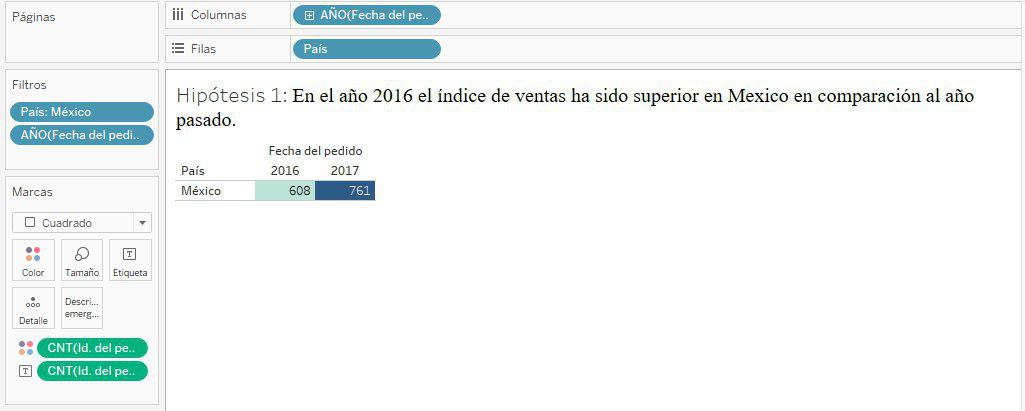
\includegraphics[scale=0.5]{imagenes/Hipotesis1.jpg} 
\end{center}

Se ha elegido este tipo de tabla “gráfica” porque se trata de mostrar un conjunto de datos muy pequeño (es una consulta muy pequeña), con lo cual, sacar gráficos con barras o en tarta puede ser excesivo, por eso se ha preferido usar una tabla con notación numérica para que se pueda entender más fácilmente.  

Tal y como podemos observar en la imagen, el resultado es antagonista a nuestra hipótesis, ya que podemos observar que en el año 2016 sólo se realizaron un total de 608 pedidos, mientras que, por el contrario, en el año 2017 tuvieron un total de 761.  

\subsection{[H2] En la temporada alta de otoño de 2017 de todos los países se registraron menos devoluciones que en el resto del año.}

\begin{center}
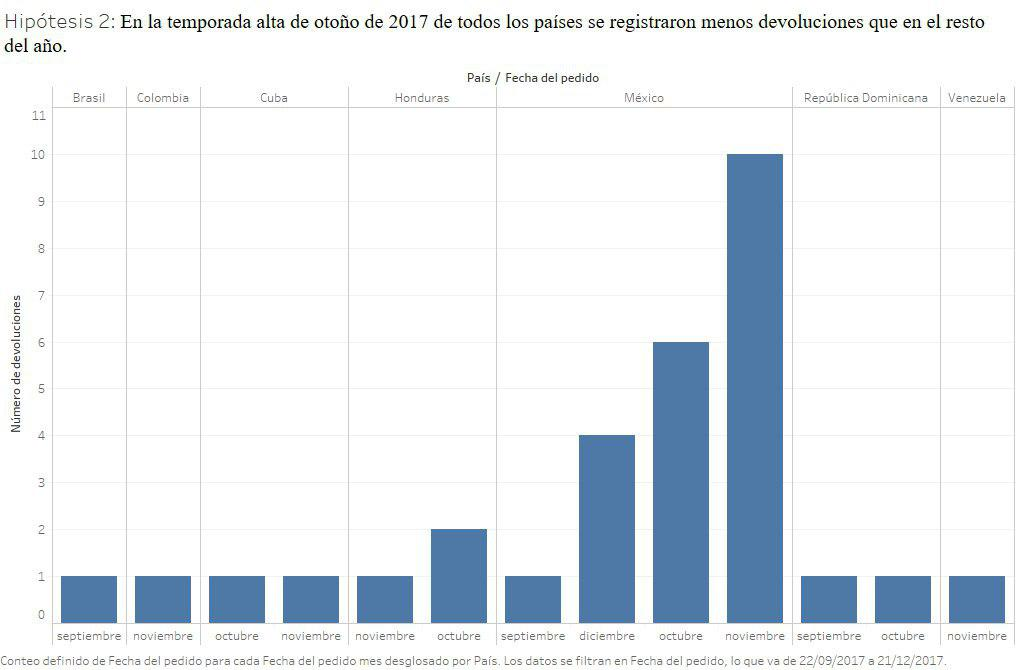
\includegraphics[scale=0.5]{imagenes/Hipotesis2.jpg} 
\end{center}

Esta tabla muestra un diagrama de barras, representando por meses y dividido a su vez por países, el número de devoluciones de productos que tuvieron lugar en la temporada de otoño. Los países que no aparecen son porque el número de devoluciones fue de 0.  

Ahora sí conviene elegir este tipo de gráfica ya que tenemos un conjunto de datos para estudiar más grande y conviene ayudar al ojo del analista cual es el valor máximo que queremos comparar.  

La siguiente gráfica muestra exactamente lo mismo, solo difiere que muestra las devoluciones en las temporadas de primavera, verano e invierno:  

\begin{flushleft}
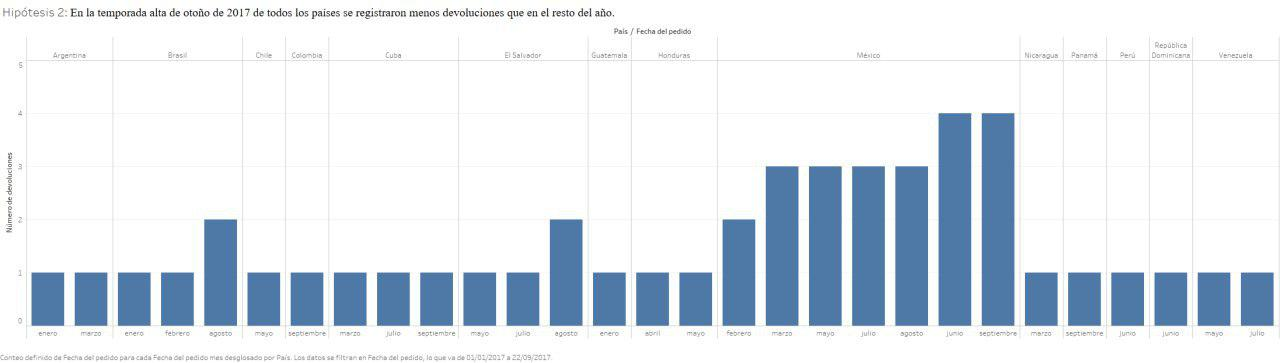
\includegraphics[scale=0.4]{imagenes/Hipotesis2_2.jpg} 
\end{flushleft}

Nuevamente nos topamos con un resultado inesperado y es que en el resto del año apenas se visualizaron devoluciones (1 devolución en casi todos los países).

\subsection{[H3] Los clientes que más han devuelto productos son de Brasil.}

\begin{center}
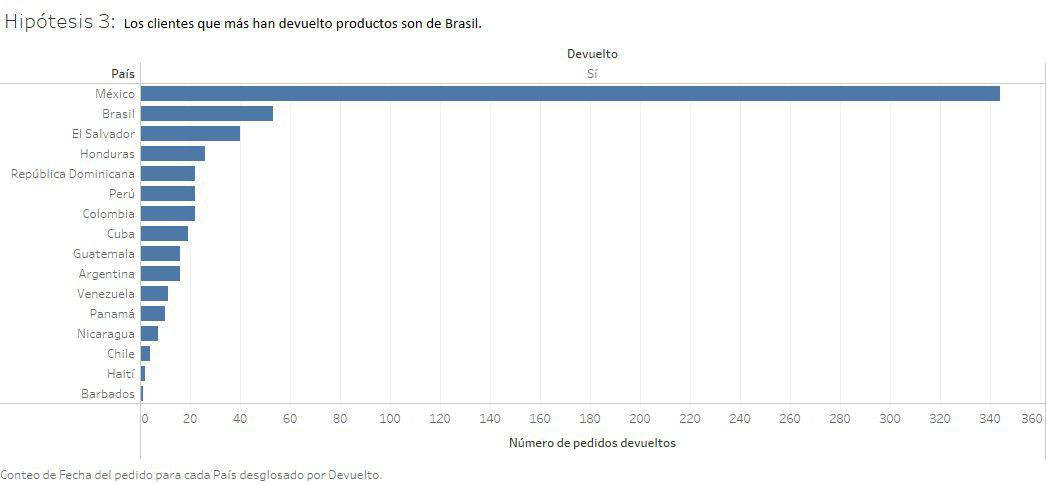
\includegraphics[scale=0.5]{imagenes/Hipotesis3.jpg} 
\end{center}

Mirando la gráfica se puede observar que el país que más productos ha devuelto es México y no Brasil (que tendría el segundo puesto).  

\subsection{[H4] En temporadas altas (comienzo de verano/navidad) los pedidos se retrasan más a la hora de enviarse.}

Para calcular el retraso en los envíos de productos, lo que se ha hecho es que se miró primero la forma de envío de cada producto, porque queremos calcular la media de cada forma de envío en esta empresa. Tenemos 4 formas de envío: urgente, rápida, mismo día y estándar. Se supone que, para envío de mismo día, no tiene que haber retrasos, pero eso es en teoría, lo comprobaremos en las gráficas. 

En esta gráfica observamos según las formas de envío los días que tarda esta empresa en mandar los productos a sus clientes. Esta media es de todos los años: 2015, 2016, 2017, 2018. Y vemos que para el mismo día de envío no hay ningún retraso, pero hay que tener en cuenta que es la media.

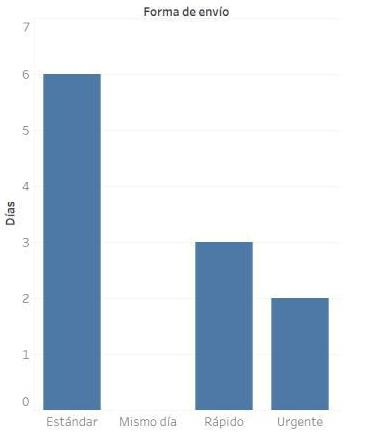
\includegraphics[scale=0.25]{imagenes/H4.jpg} 

Ya hemos sacado lo que tarda la empresa en mandar los productos. Ahora tenemos que ver las temporadas altas de pedidos según los datos que nos han sido proporcionados. También podría haberlo hecho según la experiencia y conocimiento de cultura general, pero los datos que nos han sido proporcionados son de otros países, que quizás esto puede afectar en los resultados finales. Así que también, habría que mirar las temporadas altas de pedidos: 

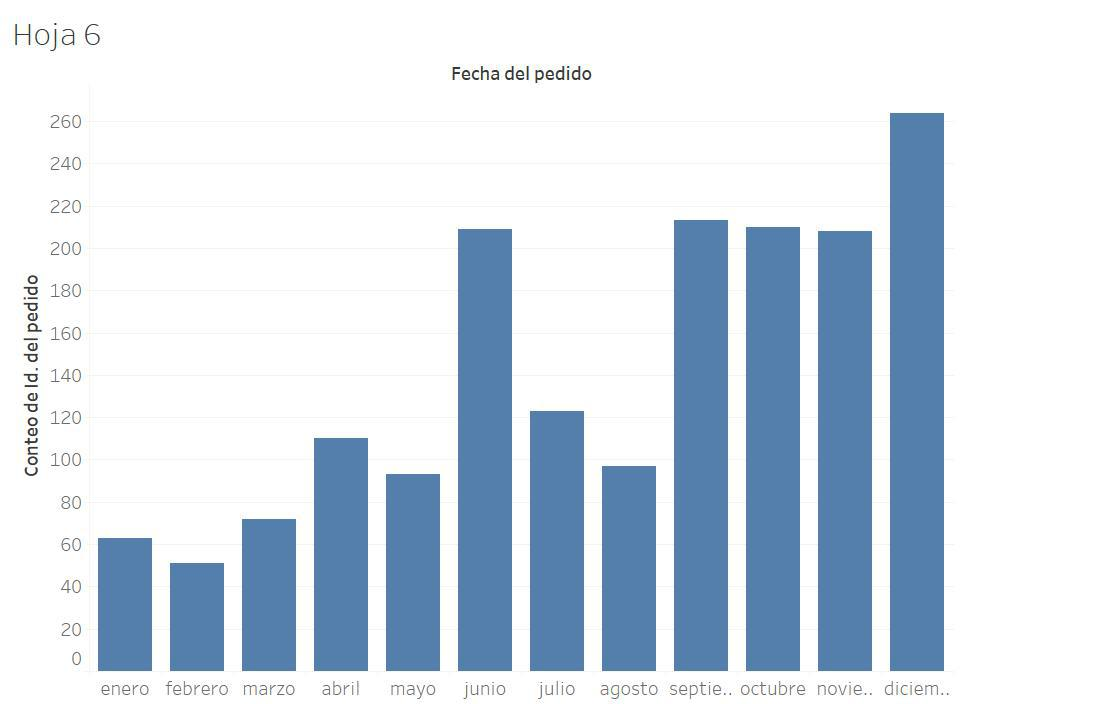
\includegraphics[scale=0.25]{imagenes/2015.jpg} 
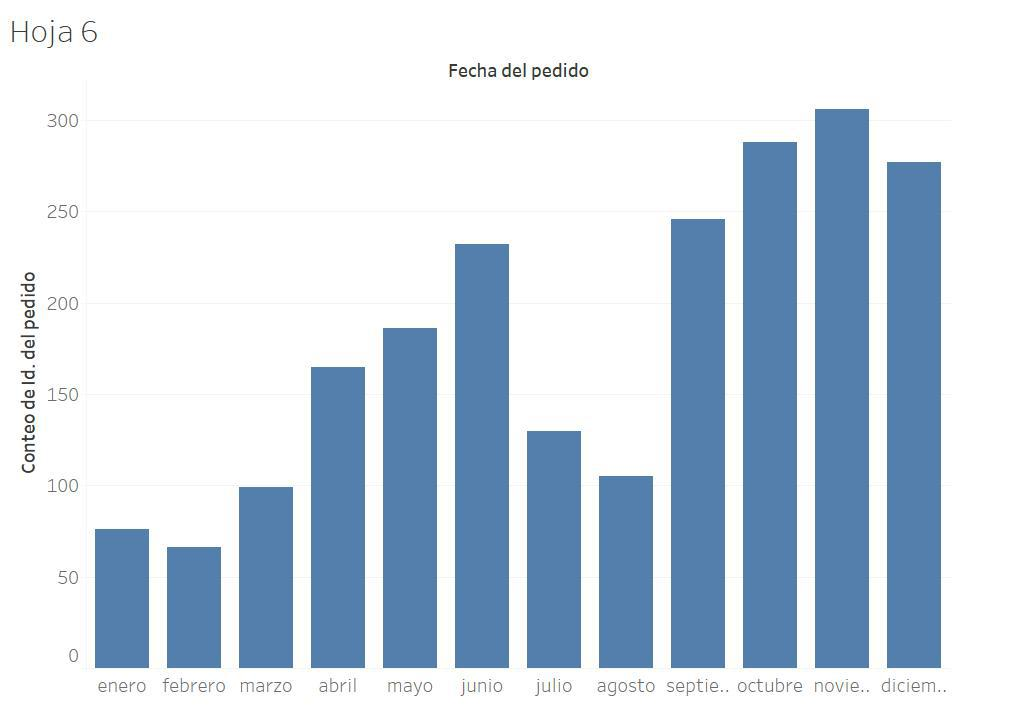
\includegraphics[scale=0.25]{imagenes/2016.jpg} 
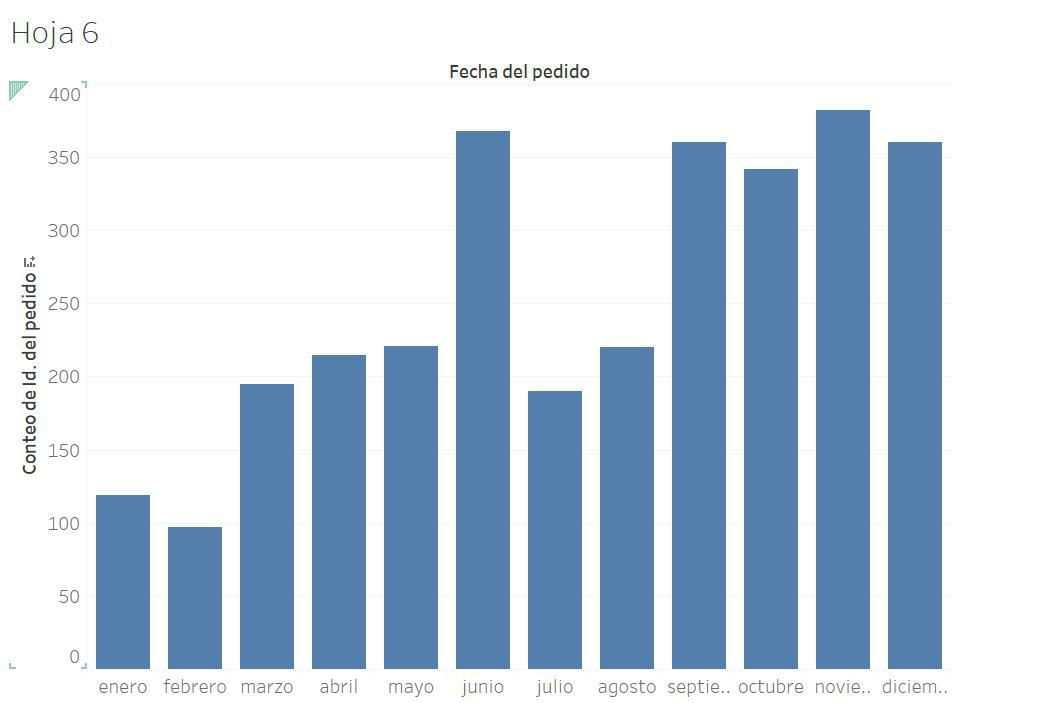
\includegraphics[scale=0.25]{imagenes/2017.jpg} 
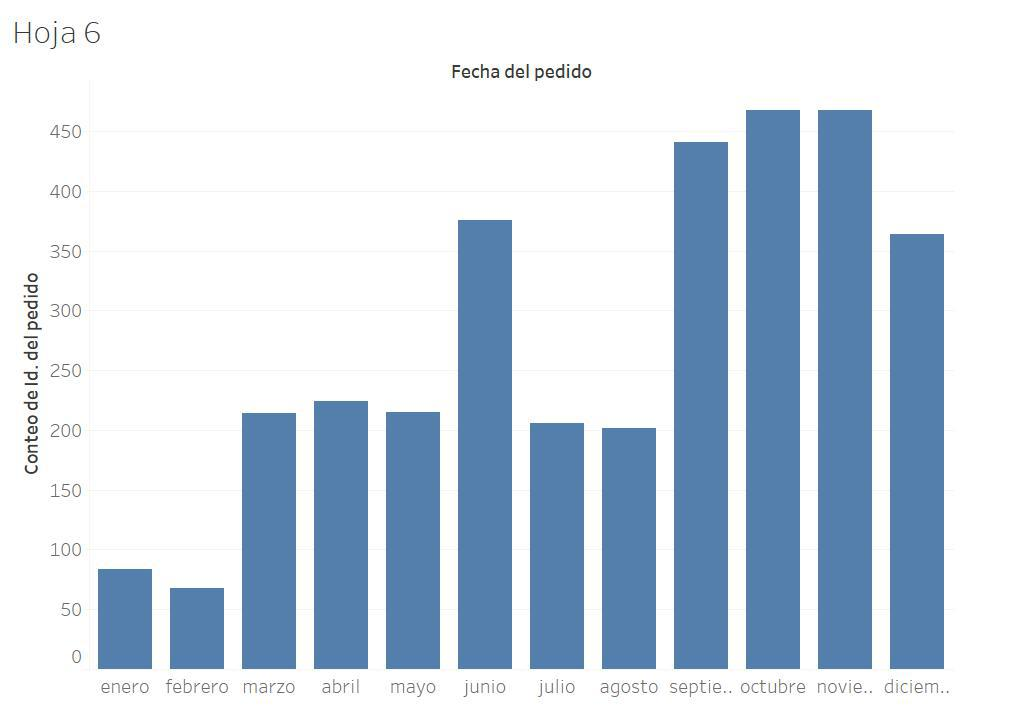
\includegraphics[scale=0.25]{imagenes/2018.jpg} 

Para 2015 vemos que temporada alta es diciembre. 
Para 2016, octubre, noviembre y diciembre.
Para 2017, junio, septiembre, octubre, noviembre y diciembre.
Para 2018, septiembre, octubre y noviembre. 

Teniendo ya la temporada alta según los años, podremos calcular el retraso y compararlo con la media.

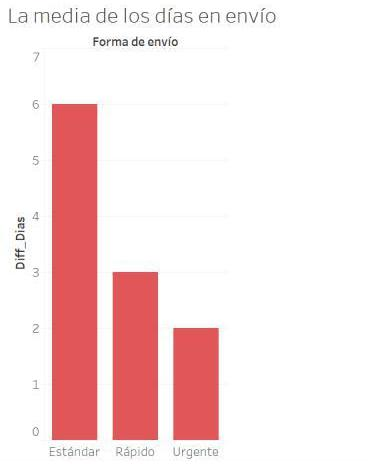
\includegraphics[scale=0.25]{imagenes/Media2016.jpg} 
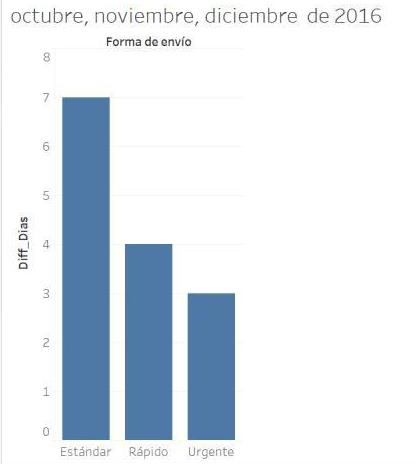
\includegraphics[scale=0.25]{imagenes/TA2016.jpg} 
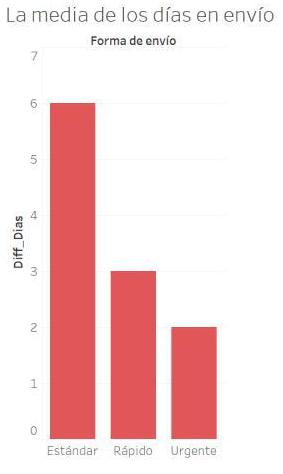
\includegraphics[scale=0.25]{imagenes/Media2018.jpg} 
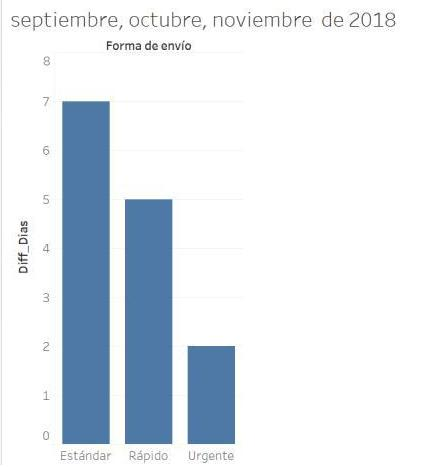
\includegraphics[scale=0.25]{imagenes/TA2018.jpg}

En 2018, se ve el aumento en 1 día para “estándar” y en 2 días “rápido”. 

Podemos corroborar la hipótesis que habíamos planteado antes. Que sí que hay retrasos en los envíos en temporadas altas.

\section{Conclusiones}

Hay que conocer muy bien los datos para poder establecer unas hipótesis que nos permitan sacar datos de utilidad para la futura toma de decisiones y esos datos deben haber sido tomados de manera correcta y organizada.

Aplicado a nuestras hipótesis, de la primera hipótesis podríamos sacar que, de un año al siguiente, México mejoró su estrategia de ventas y publicidad significativamente, propulsando sus activos gananciales gracias a la venta de más productos.

De la segunda, nos lleva a pensar justamente en la hipótesis inversa, que la temporada de otoño probablemente sea la temporada más propensa a experimentar devoluciones, aunque desconocemos los motivos (habría que realizar un análisis de mercado, análisis crítico y todo lo que dimos en la clase de teoría de esta semana, pero no disponemos de los datos suficientes en estas tablas para realizarlos).

Finalmente, de la tercera, cabría suponer que el grado de disconformidad con los productos en México es notoriamente superior al resto de países, debido quizás a un déficit de comunicación vendedor/cliente a la hora de orientar en la compra de un producto.

\begin{thebibliography}{9}

\end{thebibliography}



\end{document}